\documentclass[border=0.2cm,convert={outext=.png}]{standalone}
%\documentclass[border=0.4cm]{standalone}

 \usepackage{graphicx}
%##### English

%#### Deutsch
%\usepackage[ngerman]{babel}
%\usepackage[german]{fancyref}

%#### Usepackage #####

\usepackage{tikz} 
\usepackage{circuitikz}
\usepackage{import}
\usetikzlibrary{arrows}
\usetikzlibrary{arrows.meta}
\usetikzlibrary{shapes}
\usetikzlibrary{decorations.pathreplacing}
\usepackage[outline]{contour}
\usetikzlibrary{shadows}
\usepackage{amssymb}
\usepackage{xcolor}
\usepackage{graphicx}
\usepackage{import}
\usepackage{amsmath}
\usetikzlibrary{positioning}
\renewcommand{\familydefault}{\sfdefault}
\usepackage{pgfplots}                                                           
\usepackage{pgf}
\usepackage{booktabs,adjustbox}
\usepackage{array}

\tikzset{%
	lnk/.style={line width=5,color=black!30!white},
	joint/.style={line width=1,circle,inner sep=0.1cm,draw,fill=black!60!white},
	joint2/.style={line width=1,rectangle,minimum width=0.5cm,minimum height=0.2cm,draw,fill=black!60!white},
	lw/.style={line width=1},
	neuron/.style={circle,fill=blue!20,inner sep=0.2cm},
	neurons/.style={circle,fill=blue!20,inner sep=0.13cm},
	ex/.style = {arrows={-Triangle[length=0.12cm,width=0.18cm]},line width=1.0 },
	inh/.style={-{|[width=0.2cm]},shorten >=0.1cm,line width=1.5},
	seq/.style={arrows={|[width=0.2cm]-Triangle[length=0.12cm,width=0.15cm]},shorten <=0.1cm,line width=1.5},
	minh/.style={{|[width=0.2cm]}-{|[width=0.2cm]},shorten <=0.1cm,shorten >=0.1cm,line width=1.5},
	gj/.style={arrows={Square[open,length=0.2cm]-Square[open,length=0.2cm]},line width=1.3},
	intern/.style={circle,fill=green!20,inner sep=0.2cm},
	arr/.style = {arrows={-Triangle[length=0.15cm,width=0.2cm]},line width=1.4,color=myvio,dotted },
	comn/.style={circle,fill=nblue,inner sep=0.2cm},intern/.style={circle,fill=ngreen,inner sep=0.2cm},constn/.style={regular polygon,regular polygon sides=3,shape border rotate=180,dashed,fill=nviolet,inner sep=0.2cm},sensoryn/.style={regular polygon,regular polygon sides=3,shape border rotate=180,fill=red!60,inner sep=0.18cm},motoryn/.style={regular polygon,regular polygon sides=3,fill=norange,inner sep=0.18cm},virtn/.style={circle,fill=black!10,inner sep=0.2cm},
	cross/.style={cross out, draw=black, minimum size=2*(#1-\pgflinewidth), inner sep=0pt, outer sep=0pt},
	%default radius will be 1pt. 
	cross/.default={1pt},param/.style={cross,minimum size=0.20cm,line width=1.0},
	button/.style 2 args={
		circle, 
		minimum size=1.7cm,
		top color=#1!30!white,
		bottom color=#1,
		draw=#1!90!black,
		thick,
		append after command={
			node[circle,draw=#1!90!white,
			minimum size=1.5cm,
			font=\sffamily]at(\tikzlastnode.center)
			{\textcolor{white}{\contour{#1}{\LARGE{#2}}}}
		},
		general shadow={
			shadow xshift=.2ex, shadow yshift=-.2ex,
			opacity=.5, fill=black!50,
		}
	},
}

%#### Title page #####
\newcommand{\msize}[1]{\tiny{#1}}
%### Start of Document
\begin{document}
	
\definecolor{activegreen}{HTML}{009933}
\definecolor{ngreen}{HTML}{15a53e}
\definecolor{nblue}{HTML}{2b67c6}
\definecolor{norange}{HTML}{c99e04}
\definecolor{nviolet}{HTML}{ad13a5}
\definecolor{myvio}{HTML}{cc00cc}
\definecolor{nred}{HTML}{FF1A1A}
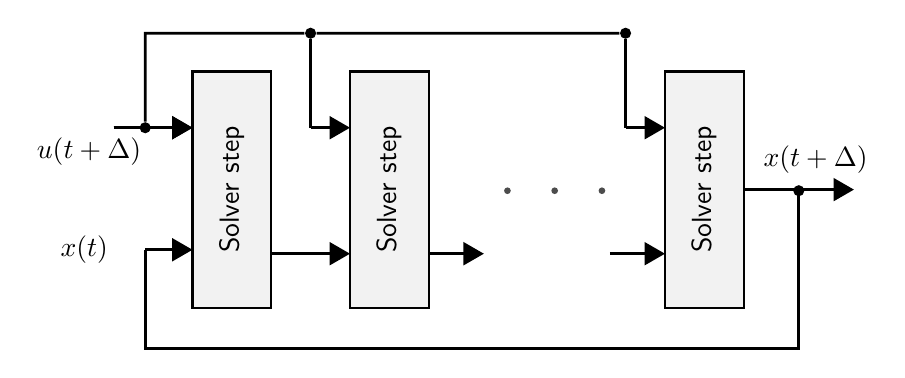
\begin{tikzpicture}
	\draw[draw=none] (-4,-2) rectangle (5,1.5);
	\node (f0) at (-3,-1.5) [anchor=west,rectangle,fill=black!5!white,draw,line width=0.8,minimum width=3.0cm,minimum height=1.0cm,rotate=90] {Solver step};
	\node (f) at (-1,-1.5) [anchor=west,rectangle,fill=black!5!white,draw,line width=0.8,minimum width=3.0cm,minimum height=1.0cm,rotate=90] {Solver step};
	\node (fe) at (3,-1.5) [anchor=west,rectangle,fill=black!5!white,draw,line width=0.8,minimum width=3.0cm,minimum height=1.0cm,rotate=90] {Solver step};
	
	\draw[-triangle 60,line width=1] (fe) to ++(1.9,0);
	\node (o) at (4.2,0) [inner sep=0.05cm, circle,fill=black] {};
	\draw[line width=1] (4.2,0) -- ++(0,-2.0) -- ++(-8.3,0) -- ++(0,1.25);
	\draw[-triangle 60,line width=1] (-4.1,-0.75) to ++(0.6,0);
	\draw[-triangle 60,line width=1] (-4.5,0.8) to ++(1.0,0);
	
	\draw[-triangle 60,line width=1] (-4.5,0.8) to ++(1.0,0);
	\node (x) at (-4.1,0.8) [inner sep=0.05cm, circle,fill=black] {};
	\node (x2) at (-2,2.0) [inner sep=0.05cm, circle,fill=black] {};
	\node (x3) at (2,2.0) [inner sep=0.05cm, circle,fill=black] {};
	\draw[line width=1] (x) -- ++(0,1.2) -- (x2) -- (x3);
	\draw[line width=1] (x2) -- ++(0,-1.2);
	\draw[line width=1] (x3) -- ++(0,-1.2);
	\draw[-triangle 60,line width=1] (-2,0.8) to ++(0.5,0);
	\draw[-triangle 60,line width=1] (2,0.8) to ++(0.5,0);
	
	\draw[-triangle 60,line width=1] (-2.5,-0.8) to ++(1,0);
	\draw[-triangle 60,line width=1] (-0.5,-0.8) to ++(0.7,0);
	\draw[-triangle 60,line width=1] (1.8,-0.8) to ++(0.7,0);
	
	
	\node at (-5.6,0.5) [anchor=west] {$u(t+\Delta)$};
	\node at (-5.3,-0.75) [anchor=west] {$x(t)$};
	\node at (5.2,0.4) [anchor=east] {$x(t+\Delta)$};
	\node  at (0.5,0) [inner sep=0.03cm, circle,fill=black!70!white] {};
	\node  at (1.1,0) [inner sep=0.03cm, circle,fill=black!70!white] {};
	\node  at (1.7,0) [inner sep=0.03cm, circle,fill=black!70!white] {};
\end{tikzpicture}


\end{document}
